\documentclass{article}
\usepackage{physics}
\usepackage{amsmath}
\usepackage{graphicx}

\graphicspath{{./figs/}}

\title{Computatonal physics - Statistical Physics}
\author{Martin Johnsrud}

\begin{document}
    \maketitle
    
    \section*{Introduction}
    By numerically integrating Newtons equation of motion og many particles, confined to a box and interacting via the Leonard-Jones potential, it is possible to see the emergence of statistical behvior like the Maxwell-Boltzmann distribution. In this exercice, we explor this behavior, and ... (more to come)

    \section*{Single particel}
        A single particel with position $\vec x = (x_1, x_2)$ in a box is modeled in a potential 
        \begin{equation*}
            V_w(\vec x) = 
            \begin{cases}
                \frac{1}{2}K(r - R)^2, & r > R \\
                0, & r < R,
            \end{cases}
        \end{equation*}
        where $r = |\vec x|$. This leads to a force 
        \begin{equation*}
            \vec F_w(\vec x) = -\nabla V_w(\vec x) = 
            \begin{cases}
                -K(r - R)\hat x, & r>R \\
                0, & r<R.
            \end{cases}
        \end{equation*}
        This equiations can the numerically integrated to simulate the trajectory of the particle. This project is done using verlet integration, 
        \begin{align*} 
            & \vec x(t + \Delta t) = \vec x(t) + \dot{\vec x}(t) \Delta t + \frac{1}{2} F\big(\vec x(t)\big) \Delta t \\
            & \dot{\vec x}(t + \Delta t) = \dot{\vec x}(t) + \frac{1}{2} \Big[\Sigma \vec F\big(\vec x(t)\big) + \Sigma \vec F\big(\vec x(t + \Delta t)\big)\Big] \Delta t^2
        \end{align*}
        Everything is done in units defined by the parametres $K, R$ and $\epsilon$, so that mass of the particle dissapears from the equations.

        
        \begin{figure}            
            \vspace{-30pt}
            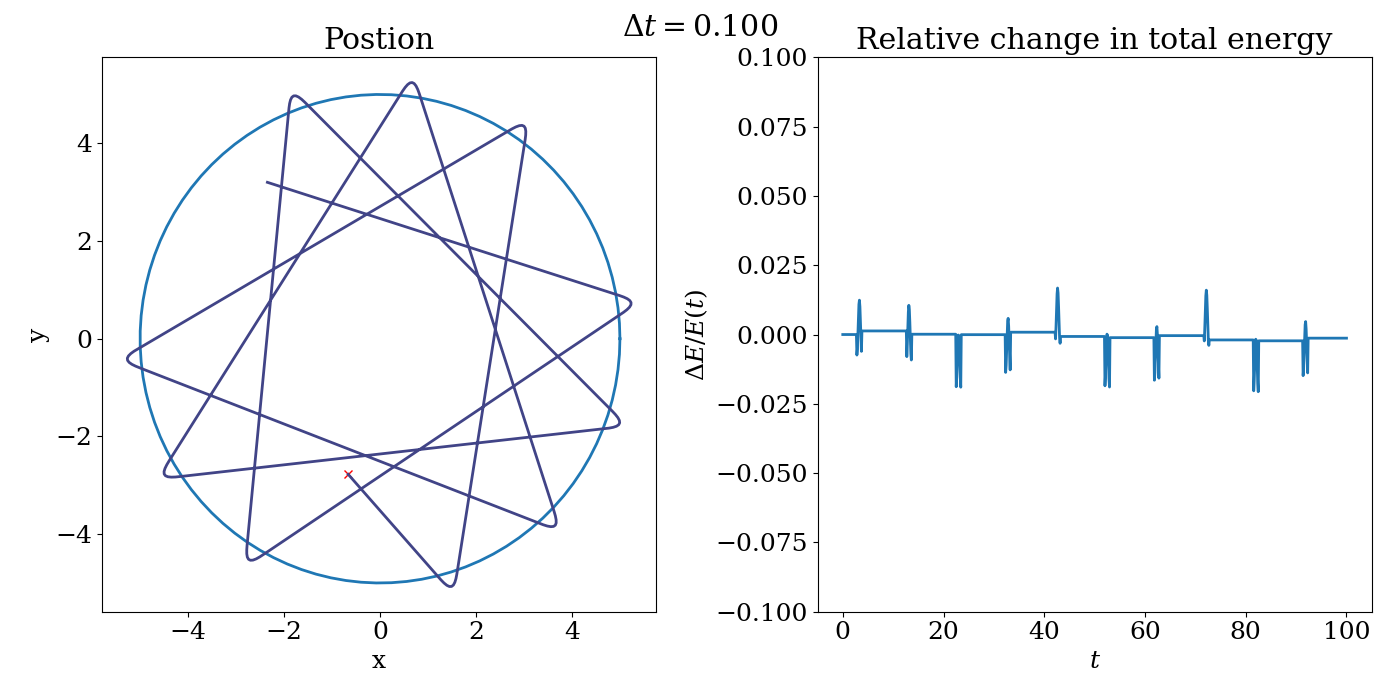
\includegraphics[width = \textwidth]{one_particle_01}
            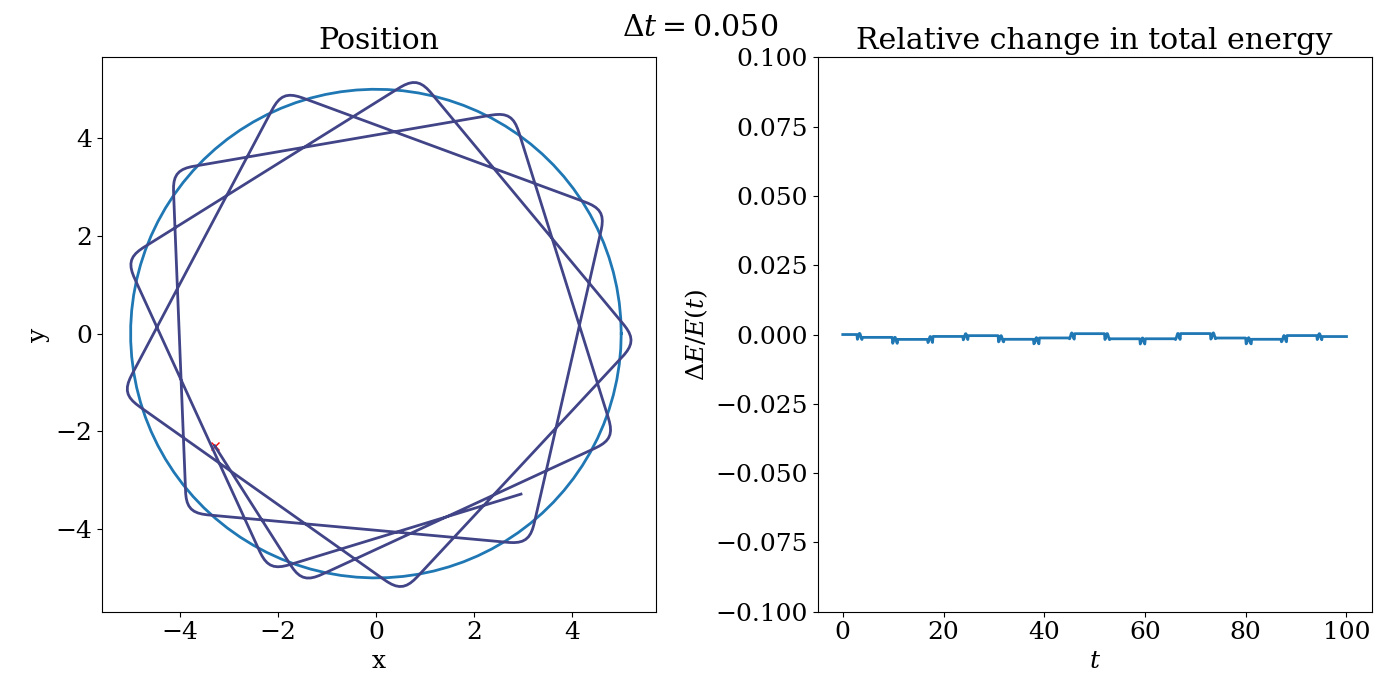
\includegraphics[width = \textwidth]{one_particle_005}
            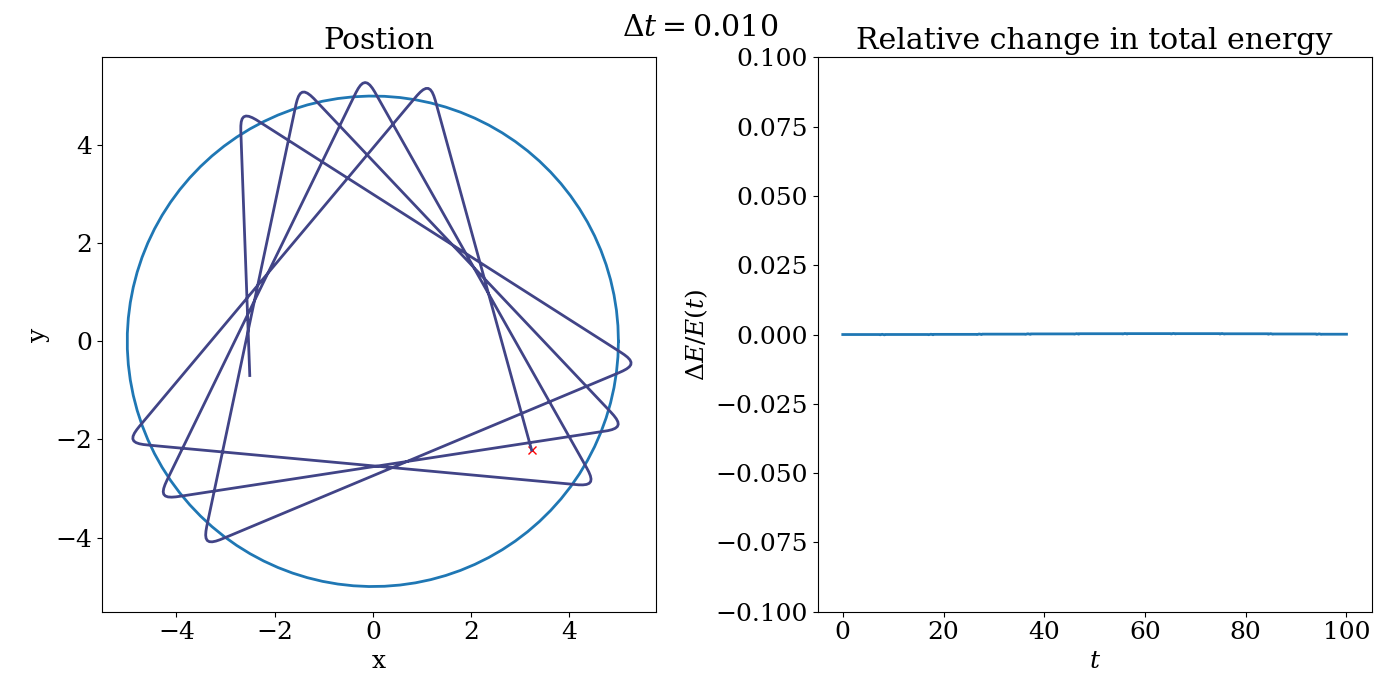
\includegraphics[width = \textwidth]{one_particle_001}
            \caption{The figure shows the path of a particle in the potential described in the text, integrated using different steplengths. The right side shows the relative change in energy of the particle, as a function of time. The red x marks the starting position of the particle.}
            \label{task 1}
        \end{figure}

        \paragraph*{}
        Figure \ref{task 1} shows simulation series of one particle in a box, using different steplengths. The energy of the particle can be used to assess the accuracy of the particle. As there are noe dissipative forces, energy is conserved. Accurate simulations should then have very small changes in energy, $\delta E - E(0)$, relative the starting energy $E(0)$. This is plotted to the right in figure \ref{task 1}. $\Delta t = 0.01$ seems to yield sufficient accuracy, and wil be used throughout this exercise.
        

    \section*{$N$ particles}
        When moddeling $N$ particles $\{ \vec x_k\} = \{ (x_1^{(k)}, x_2^{(k)}) \}$, each one of them is subject to the force from the potential $V_w(\vec x_k)$, as well as a modified Leonard-Jones potential the interaction potential. The potential felt by particle $k$ is then
        \begin{equation*}
            V_k(\vec x_j) = 
            \sum_{r_{kj}<a}\epsilon \bigg[ \bigg( \frac{a}{r_{kj}}\bigg)^{12} - 2\bigg(\frac{a}{r_{kj}}\bigg)^{6} + 1 \bigg]
        \end{equation*}
        Here, $r_{kj} = |\vec x_k - \vec x_j|$. The force on particel $k$ by this potential is
        \begin{equation*}
            F_k (\vec x_j) = -\nabla_k V(\vec x_j) = \sum_{r_{kj}<a} 12 \epsilon \bigg[ \bigg( \frac{a}{r_{kj}}\bigg)^{12} - \bigg(\frac{a}{r_{kj}}\bigg)^{6}\bigg] \frac{\hat x_{kj}}{r_{kj}},
        \end{equation*}
        where $\hat x_{kj} = (\vec x_k - \vec x_j) / r_{kj}$. This is, like in the case with one particle, simulated using verlet integration, only now using the force.
        \begin{equation*}
            \Sigma \vec F_k = -\nabla_k \big( V_w(\vec x_k) + V_w(\vec x_j) \big).
        \end{equation*}

        \begin{figure}
            
            \vspace{-16pt}
            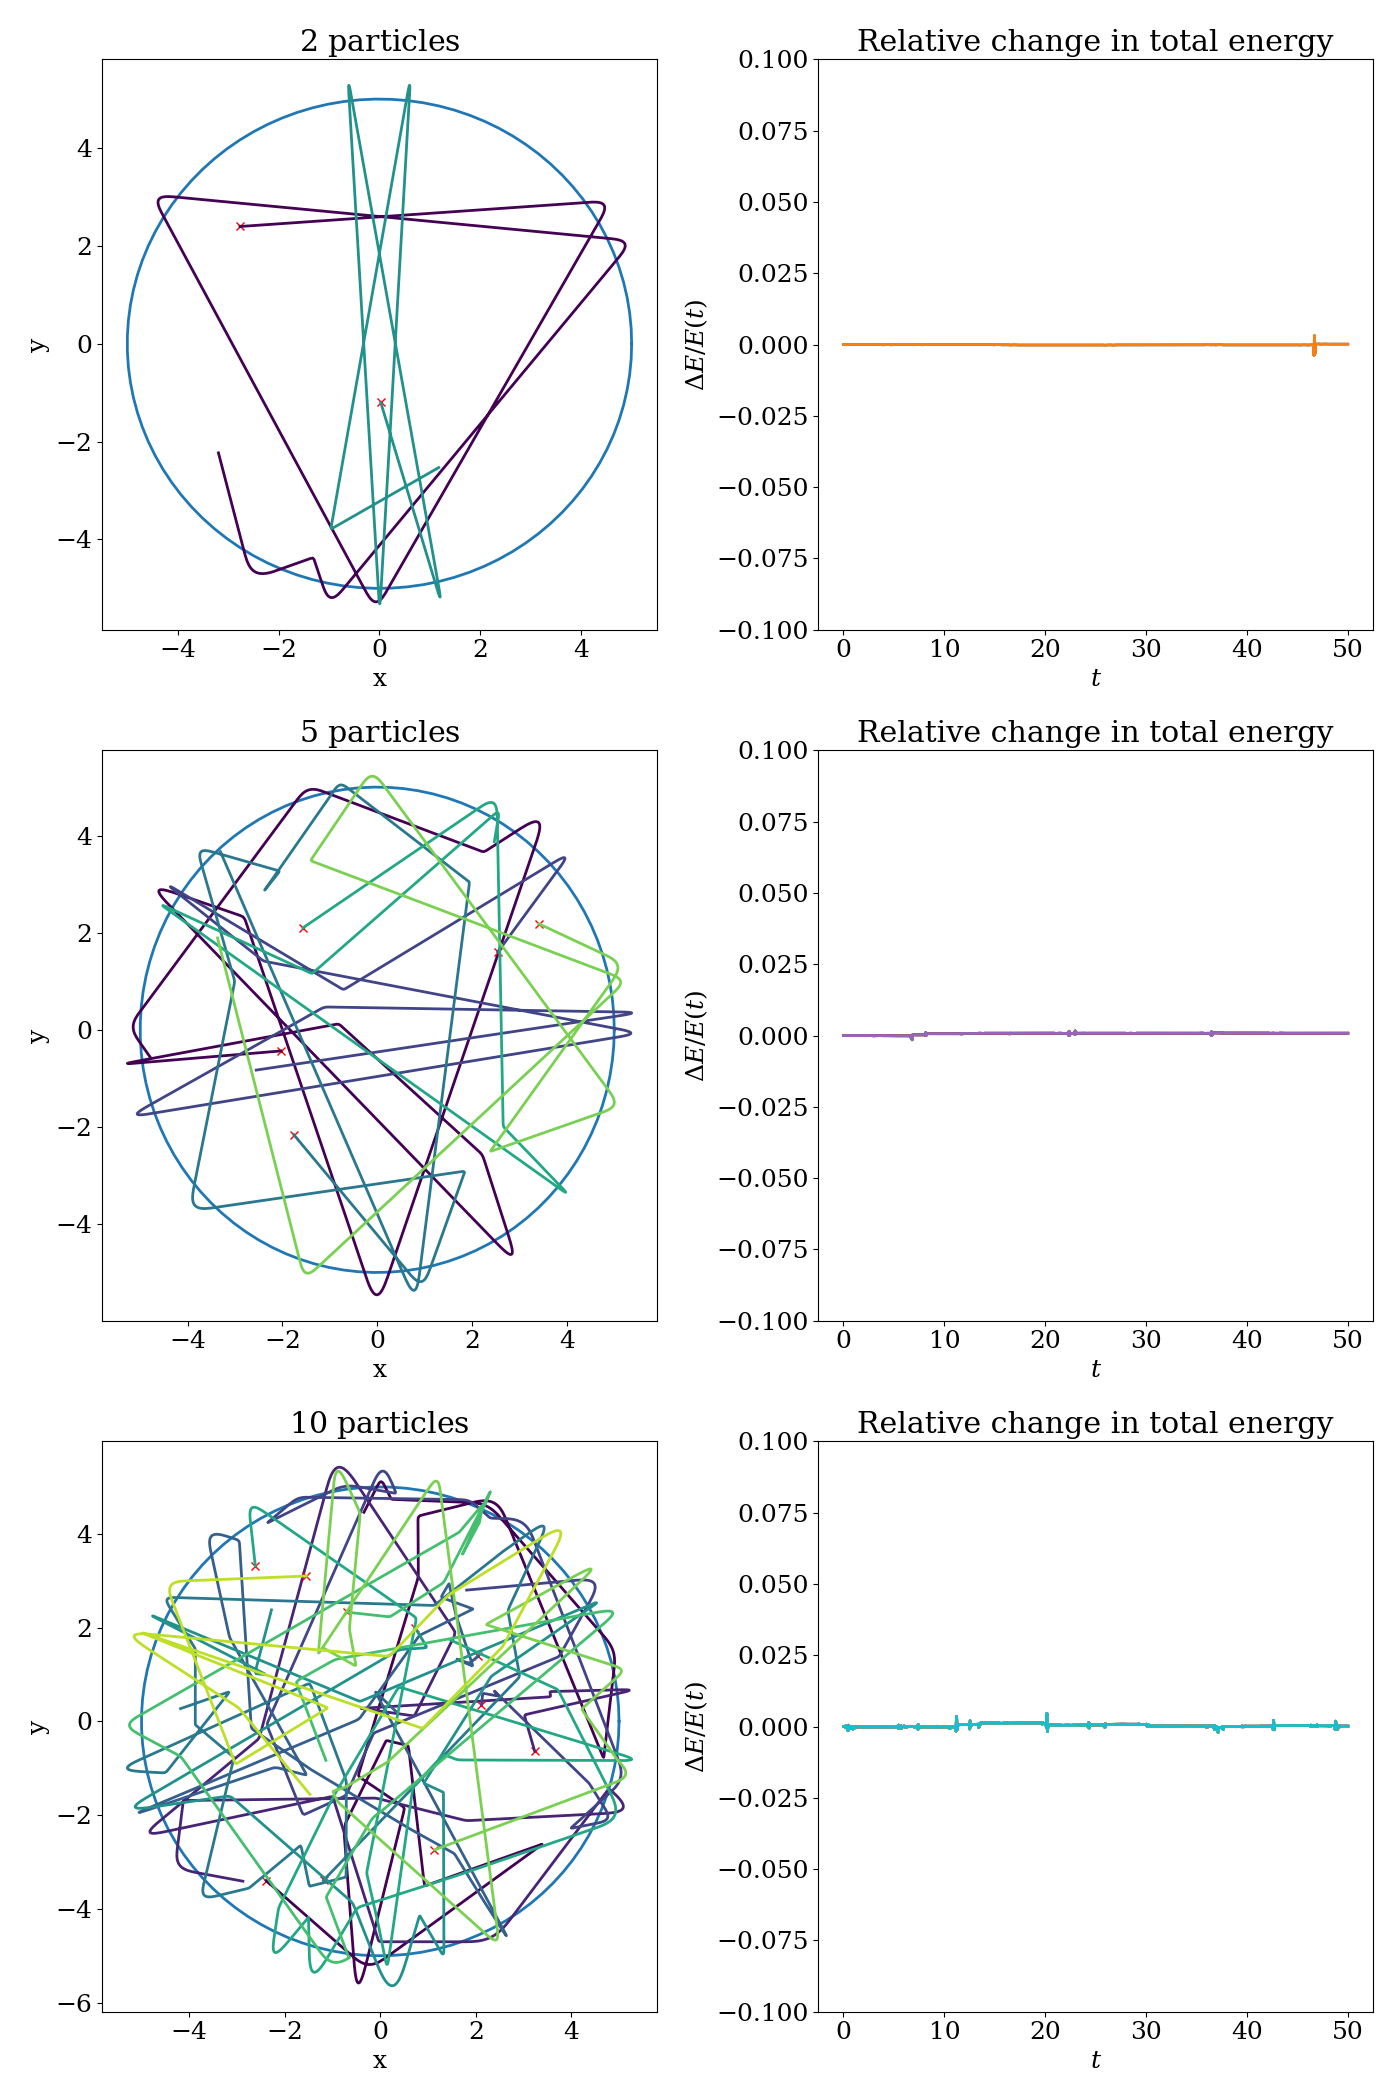
\includegraphics[width = \textwidth]{several_particles}
            \caption{On the left, the path of different numbers of particles are shown. On the right, though there are som jumps in total energy, it is very close to conserved, giving confidence to the model.}
            \label{several particles}

        \end{figure}

        \begin{figure}
            
            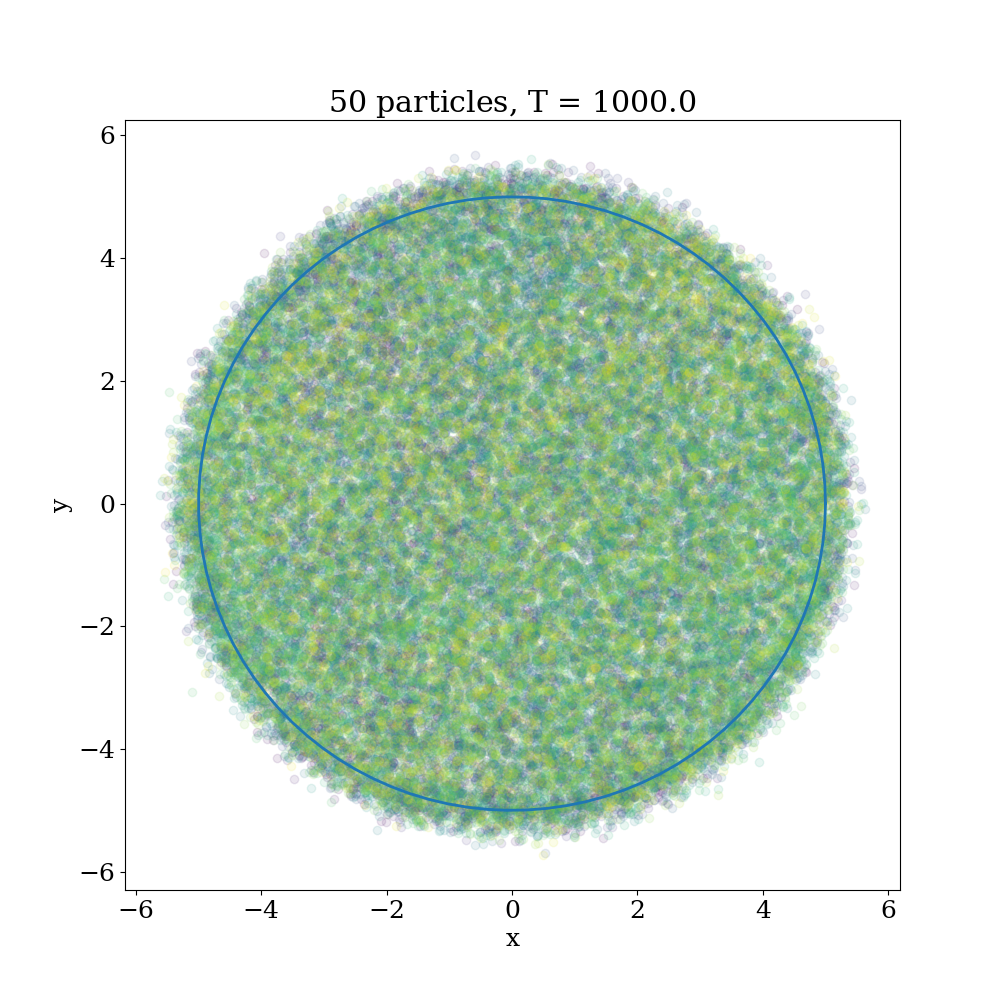
\includegraphics[width = \textwidth]{scatter}
            \vspace{-30pt}
            \caption{A scatter plot of the position of $50$ particles, each with $1000$ datapoints shown. Different particles have different collor, showing that the particles get mixed.}
            \label{scatter}

        \end{figure}

        \paragraph*{}
        Figure \ref{several particles} shows the simulation of particles with interactions implemented, as well as how the relative shifts in total energy in the total energy. It is evident that the system immediately becomes chaotic, and the ergodic hypothesis seems much more plausible. This becomes even clearer in figure \ref{scatter}, showing a scatter plot of the position of $50$ particles over a time $T = 1000$. 

\end{document}